\chapter{热类木星统计性质} \label{chapter:data_stat}

\section{系外行星统计列表}

在引言部分 \S \ref{sec: exopftheory},我们曾提到在如今已探测的系外行星中,有一群周期
小于十天却拥有大于土星质量的行星种群,被称为热类木星\footnote{若按照热类木星的定义,
其准确叫法应为近距离类木星,因为行星的有效温度不仅仅与主星的距离有关,而且还与主
星的有效温度有关。}。为了研究此类行星的统计性质,本文汇总了知名的四大系外行星数据
库网站 \url{http://exoplanets.eu/}、\url{http://exoplanets.org/}、\url{http://
exoplanetarchive.ipac.caltech.edu/} 和 \url{http://openexoplanetcatalogue.com/} ,并整理出
比较统一规范的系外行星列表\footnote{\url{https://github.com/EXONJU/ExoPlanetList}}。如
图 \ref{fig:hrplanet} 与 图 \ref{fig:exoskydist} 所示,在这行星数目为 3701 的样本中,共有 
375 颗系外热类木星系统(后文简称 HJs)。系外行星在南北天球分布并没有太多不均匀性
(除了巡天观测密集的几个区域以外),而 HJs 却在巨星分支中出现概率偏小(在 \S 
\ref{sec:hjofgiants} 中讨论),且大多数集中在类太阳恒星周围(下文介绍此为观测选择效
应)。本章节后续分析将统一建立在此 HJ 列表的范畴内讨论。

\begin{figure}
\centering
\includegraphics[width=1.0\textwidth]{figures/chapter4/fig2_HRplanet.pdf}
\caption{已确认系外行星的色指数与光度分布图,墨蓝色点为伊巴古星表临近太阳 150 pc 以内的恒星(图 \ref{fig:hrdiagram}),红五角星为太阳,绿色与黄色点如图 \ref{fig:exoskydist},被探测到的系外行星以及热木星明显集中在类太阳恒星附近,为观测选择效应。}
\label{fig:hrplanet}
\end{figure}


\begin{figure}
\centering
\includegraphics[width=1.0\textwidth]{figures/chapter4/fig1_exodistmollweide.pdf}
\caption{已被确认的系外行星在赤道坐标下的天球分布。图中蓝色虚线为银道面,可以看到巡天一般会远离银盘面(CoRoT 与 OGLE 除外)。绿色点为所有行星,黄色点则为热木星,点大小正比于 V 波段星等,从此图未见南北天的观测选择效应,$Kepler$ 视场(RA=19h 22m 40s,Dec=+44$^\circ$ 30' 00'' )为已确认系外行星最密集的区域之一。}
\label{fig:exoskydist}
\end{figure}


\section{HJs 出现概率}  \label{sec:hjoccurate}

按照已有的数据,现今探测到的 HJ 总数目约占已确认行星的 10\% 之多,这也是为什么
在图 \ref{fig:exomassper} 中,明显可以观察到一群质量在木星质量周期小于十天的行星
族。然而这与观测的选择效应密不可分。一个完备的统计必须建立在限定体积样本(
Volumn-limited sample)之上(文献 \citen{WinnFabrycky2015})。在一个限定体积的样
本中,热木星出现的概率并不高。Cumming 等人于 2008 年对 RV 巡天中的 600 颗 FKGM 
恒星监测了 8 年后的结果显示\cite{Cumming2008},对于 $M_\tif{p} > 100 \tif{M}_\oplus,\, 
P<5.5$ years 的行星的出现概率可用如下公式描述:

\begin{equation} \label{eq:pltoccurate}
\frac{\tif{d} N}{\tif{d}\ln M_\tif{p} \tif{d}\ln P} \propto  M_\tif{p}^\alpha P^\beta \ \, ,
\end{equation} %myequation{行星出现数目的概率分布}
其中指数 $\alpha = -0.31 \pm 0.20 $,$\beta = 0.26 \pm 0.10$。结合其他种类的巡天项目,
对应的 HJs 的出现概率大致为 0.5 \% 到1.5 \% 之间不等\cite{Howard2012,Marcy2005,
Mayor2011,Wright2012}。此概率的不同和恒星的星族选择密切相关\cite{Wright2012},比如
恒星的金属丰度和类木星出现的概率有明显的正相关性\cite{Gonzalez1997,Santos2001,
Santos2004,Fischer2005,Udry2007,Sozzetti2009,Sousa2011},这也恰好佐证了 \S 
\ref{sec:clspftheory} 中描述的气巨星重元素核吸积模型。


\section{HJs 形成} \label{sec:hjform}


在传统的核吸积模型中\cite{IdaLin2004b},气巨星往往需要在距离主星几个天文单位的地方
才能有足够多的原材料(绝大部分由冰组成)供固态核形成。然而在观测中,HJs 的统计
分布于 3 天附近存在峰值(见图 \ref{fig:hjperecc})。因此需要解释 HJ 的形成,大致上有
两大种方法:在传统的行星形成基础上引入木星的轨道迁移(\textit{orbital migration})或
直接于当地形成(\textit{in situ. formation})。关于热木星的本地形成请参见文献 
\citen{Batygin2016},本文分析的主要讨论对象为前者。

\begin{figure}[t]
\centering
\includegraphics[width=1.0\textwidth]{figures/chapter4/fig3_peccdist.jpeg}
\caption[热类木星系统的周期与轨道偏心率分布图。可以看到系外行星样本(未经过选择效应修正)在三天周期分布达到热类木星的峰值,虚线为类太阳恒星周围行星拥有近心点距离 $a(1-e) = 0.03$ AU 的轨道。右侧图为 SB9 光谱双星星表的类似分布图,图片取自 Winn 和 Fabrycky。]{热类木星系统的周期与轨道偏心率分布图。图片取自文献 \citen{WinnFabrycky2015},可以看到系外行星样本(未经过选择效应修正)在三天周期分布达到热类木星的峰值,虚线为类太阳恒星周围行星拥有近心点距离 $a(1-e) = 0.03$ AU 的轨道。右侧图为 SB9 光谱双星星表的类似分布图。}
\label{fig:hjperecc}
\end{figure}


\subsection{轨道迁移}

在传统的行星形成的基础上,行星的轨道迁移并不需要引入额外的行星核心生长以及气体
吸积机制。轨道迁移代表着轨道半长径 $a$ 发生了变化,在椭圆二体运动中行星的角动
量与能量拥有如下表达式(本文内均假设 $M_\tif{p} \ll M_\tif{s}$):

\begin{eqnarray}
E = - M_\tif{p} \, \frac{\mu}{2a} \\ \label{eq:2be}
J = M_\tif{p} n a^2 \label{eq:2bam}
\end{eqnarray} %\myequation{二体运动中的能量与角动量}
其中 $n$ 为平均轨道角速度,满足开普勒第三定律 $n^2a^3=\mu$,其中$\mu = G M_\tif{s}$
如此轨道迁移势必意味着角动量(Angular Momentum,简称 AM)与能量的交换,因此必须
有其它物体与行星之间发生 AM 与能量传递。这样一来,我们又可将轨道迁移大致分为两
种情况:气体盘迁移(\textit{disk migration})和高偏心率迁移(\textit{high-e migration})。

\subsubsection{气体盘迁移} \label{sec:diskmig}

由于木星质量的行星核心形成后会依然嵌套在恒星周围的气体盘内,因而由于盘的气体和之
间会存在 AM 交换。这样的的 AM 交换通常是通过处于 Lindblad 共振的气体的 Co-
rotational 力矩来实现\cite{Binney1987,GoldreichTremaine1979},比如土星环的结构
\cite{GoldreichTremaine1980}。简单来说第 $m$ 阶共振距离主星半径与行星轨道之间的关系
为 $r_\tif{L} = (1\pm 1/m)^{2/3} a_\tif{p}$。在二体问题中希尔半径(或洛希半径)可描述为:

\begin{equation} \label{eq:hillradius}
r_H = \big( \frac{M_\tif{p}}{3M_\tif{s}} \big) ^{1/3}
\end{equation} %myequation{希尔半径(或洛希半径)表达式}

如果行星的质量足够大,使得希尔半径大于盘的标高($r_H > h$),那么盘可能被被打开缺
口。与此同时,由于气体盘的粘性,此缺口也可能被气体重新填上。1986 年,Lin 等人通过
比较盘缺口由于粘性重新被填补上以及由于 Lindblad 共振又再被打开的时标,得出在经典的
原行星盘参数下,木星质量的行星足以打开空缺,而土星的质量则约为打开空缺的临界值
\cite{Lin1986,Ward1997}。后来该理论被成功地在人类发现的第一颗类太阳系外 HJ --- 51 Peg
 b 上\cite{Lin1996},比如在 5 AU 附近的木星,在标准的行星盘打开缺口后,将在时标为 0.5 
 Myr 左右迁移至原行星盘的内边界。这样的气体盘迁移又被称作第二型(Type II)轨道迁移
 (见图 \ref{fig:diskmig})。

\begin{figure}[t]
\centering
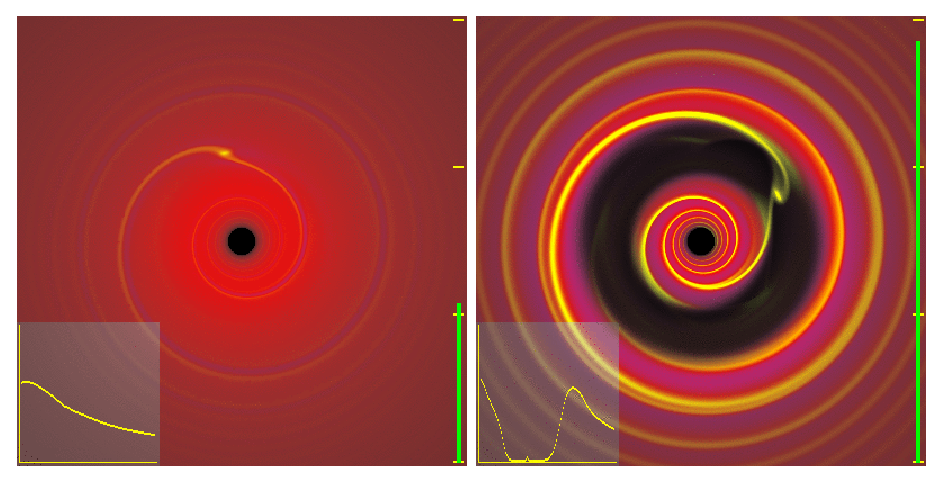
\includegraphics[width=1.0\textwidth]{figures/chapter4/fig3_diskmig.eps}
\caption[典型的第二型轨道迁移数值模拟,大质量行星可以在盘内打开空缺,并且往靠近恒星的盘内侧迁移。图片版权 Armitage\/Rice。]{典型的第二型轨道迁移数值模拟,大质量行星可以在盘内打开空缺,并且往靠近恒星的盘内侧迁移。图片取自文献 \citen{Armitage2005}。}
\label{fig:diskmig}
\end{figure}


\subsubsection{高偏心率迁移} \label{sec:highemig}

行星在气体盘中的迁移往往会受气体的阻尼作用而不那么剧烈(保持小偏心率轨道来交换
AM)。相比之下,其它天体造成的引力扰动则会显得更为直接,之所以称此类作用为
高偏心率迁移也正是如此得名。一旦类木星的偏心率达到能使得其轨道近心点距离达到当
前观测 HJs 几天轨道周期的位置,那么潮汐演化便可将其作用成热木星(\S \ref{sec:tidal})。
高偏心率作用的天体可以是一群小天体(单个小质量的天体几乎不能改变木星),如散射
星子盘导致的行星迁移\cite{Malhotra1993,Murray1998,Morbidelli2007,Thommes2008},
或者更多的则是质量相当或更大天体的强引力扰动(如木星与土星的长期摄动
\cite{MurrayDermott1999ssd})。目前此类别下主流的解释因素包括以下几种:

\textbf{伴星级扰动}。早在 1962 年,木星的存在对高轨道倾角太阳系小天体的轨道影响就
已被提出\cite{Lidov1962,Kozai1962}。而后 Wu 和 Murray 于 2003 年将此 Lidov-Kozai 
效应效应引入解释系外热木星\cite{WuMurray2003},即当引入一颗行星系统外具有较大
轨道倾角的伴星时,行星的轨道偏心率(以及轨道倾角)会发生周期性的 Kozai 共振
\cite{Innanen1997}。然而观测中伴星存在的概率是否能解释所有的 HJ 系统\cite{Wu2007,
Fabrycky2007},共振的最高偏心对伴星的质量和轨道要求也值得进一步讨论\cite{
Naoz2011,Nagasawa2011}。甚至在恒星形成的星团环境中,其它天体的飞掠(flyby)也
可能会对行星系统造成一定的影响\cite{Spurzem2009}。

\textbf{行星级扰动}。多行星系统内行星之间无处不存在着扰动,如果行星之间动力学足够
不稳定,那么可能发生行星---行星散射(planet-planet scattering 简称 PPS,参见文献
\citen{Rasio1996a})。对于一般有规律并排(orderly spaced)的行星系统,动力学作用
会产生中等偏心率的行星\cite{Zhou2007,IdaLin2013,Lin1997,Juric2008,Chatterjee2008},
而若要产生能够形成 HJs 的大偏心率,则需要长期作用下的混动效应\cite{Wu2011}。

另外,形成热木星高偏心率还有一些混合以上盘迁移以及高偏心率迁移的其他理论,详见
文献\citen{Weidenschilling1996,Nagasawa2008,Chen2013}。理论虽多,但迁移的总体思
路实则不变: 拥有能够与 HJ 交换 AM 的另外一颗天体以及整个系统初始的角动量亏损
(Angular Momentum Deficit,AMD)。正是如此才需要观测和统计去区分不同的物理作
用过程并且打破观测中不同理论的简并度(图 \ref{fig:pfenv})。


\section{引力潮汐作用} \label{sec:tidal}

前文提到在高偏心率迁移的框架下,需要额外引入潮汐过程才能解释如今观测到 HJs
几乎全体近圆的轨道统计分布(见图 \ref{fig:hjperecc})。在 51 Peg b 发现的第二年,
Rasio与 Ford 就意识到潮汐因素在 HJs 的形成演化中起了非常重要的作用\cite{Rasio1996b}。
而事实上,在近距离的二题问题中(轨道周期在几天附近),由于天体并非质点,因而
引力潮汐导致的形变效应的确是一项不可忽略的非开普勒(non-keplerian)作用项。潮
汐现象在我们太阳系甚至地月系统都很常见,月球的公转自转潮汐锁定,以及地球上海洋
的涨潮落潮,也都是潮汐的体现。现代的潮汐理论主要基于 Darwin 在 1880 年基于球谐函
数下对天体非开普勒引力势展开\cite{Darwin1880}:

\begin{equation} \label{gravipotential}
U(r) = \sum\limits_{l=2}^\infty \sum\limits_{p=0}^l\sum\limits_{q=-\infty}^\infty \frac{Gm}{a} A_{l,p,q}(e,\,\Psi)\big(\frac{r}{a}\big)^l Y_l^p(\theta,\,\phi) \tif{e}^{-\tif{i}q n t} \ .
\end{equation} %\myequation{非球形引力势展开}
各物理量的定义如图 \ref{fig:tideillu} 所示,$n$ 为平均轨道角速度,$a,e$ 为轨道根数
(有时也会用二体之间的距离 $d$ 来作为展开基数),$\Psi$ 为 $m$ 体轨道法向 $L$ 
与 $M$ 体自转法向的夹角( 又称 obliquity),$A_{l,p,q}$ 系数则依赖于天体 $m$ 的轨
道,对应的潮汐力矩以及能量耗散均可从上式得到(参见综述 \citen{Ogilvie2014})。


\begin{figure}[t]
\centering
\includegraphics[width=1.0\textwidth]{figures/chapter4/fig4_tides.pdf}
\caption{引力潮汐形变示意图,其中 ($r,\,\theta,\,\phi$) 是以中心天体赤道为基准面的球坐标参考系。$L,\,S$ 分别为扰动体 $m$ 的轨道角动量与潮汐形变体 $M$ 的自转角动量。为了显示,此图的潮汐鼓包被大大地夸张了,并且没有考虑 $M$ 自转产生的鼓包。}
\label{fig:tideillu}
\end{figure}

在上面描述的基础上,如果将潮汐展开精确到二阶($l=2$),并且取角向模数$m,n = 0 $,
便可得到最常用的平衡潮汐(equilibrium tide)模型的近似解。此时形变天体可以用常数滞
后角度(constant phase lag)或滞后时间来参数化描述复杂的潮汐模型:

\begin{equation} \label{eq:eqtide}
Q^{-1}=\frac{1}{2\pi E_0} \oint \big( -\frac{\tif{d} E}{\tif{d} t}\big)\,\tif{d} t = \tan 2\delta \ ,
\end{equation} %\myequation{平衡潮汐模型下的 $Q$ 参数}

Goldreich 和 Soter 于 1966 年将上述模型用在计算太阳系内行星的潮汐耗散率中
\cite{Goldreich1966},同样的理论也用在近距离双星潮汐演化中\cite{Hut1981,Zahn1977}。
对于系外行星而言,HJs 的产生和演化包括两个过程:行星的轨道圆化(circularization)
以及两个天体的轨道自转同步过程(synchronization)。其中每个过程恒星与行星的物质
组成以及内部结构都会影响能量耗散和角动量交换效率,在弱摩擦假设下的平衡潮汐模型
则采用 $Love$ 数 $k_2$ 来描述不同的物质耗散结构。


\section{Rossiter-McLaughlin 效应} \label{sec:rmeffect}

\begin{figure}[b!]
\centering
\includegraphics[width=1.0\textwidth]{figures/chapter4/fig5_RMsim.pdf}
\caption[系外行星 Rossiter-McLaughlin 效应示意图。由于行星在凌星过程中遮挡主星的部分区域从而导致主星红移与蓝移的相应部分减小,图中不同的自转---公转倾角以及影响因子均会影响到 RM 效应的视向速度曲线波动轮廓,本图版权 Gaudi/Winn。]{系外行星 Rossiter-McLaughlin 效应示意图。由于行星在凌星过程中遮挡主星的部分区域从而导致主星红移与蓝移的相应部分减小,图中不同的自转---公转倾角以及影响因子均会影响到 RM 效应的视向速度曲线波动轮廓,本图骄傲地取自文献\citen{Gaudi2007}。}
\label{fig:rmsim}
\end{figure}

Rossiter-McLaughlin 效应(RM 效应)最早可能是被 Holt 于 1893 年预言并在双星中观测
证实\cite{Holt1893}。后来 Rossiter 与 McLaughlin 分别详细描述了此过程,并且常常被引
用为 RM 效应\cite{Rossiter1924,McLaughlin1924}。在原理上如果一个天体遮挡住另一天
体,那么背景天体的光谱的视向速度的蓝移与红移部分会分别被遮挡,从而造成视向速度在
掩食内有如下振幅的波动:

\begin{equation} \label{eq:rvdvofrm}
\Delta V_\tif{RM} = (R_\tif{p} / R_\tif{s})^2 \sqrt{(1-b^2)} \, v\sin i
\end{equation} %\myequation{RM 效应的视向速度波动振幅}
其中 $(R_\tif{p} / R_\tif{s})^2$ 约为凌星深度,$b$ 为凌星最大时刻两天体之间的距离影响
因子,$v\sin i$ 为主星的空间投影自转速度。图 \ref{fig:rmsim} 所示为不同的 $b$ 与 
$\lambda$ 参数下恒星视向速度的理论波动,$\lambda$ 在系外行星领域被称作投影行星
轨道法向与恒星自转轴夹角(后文统称自转---公转夹角),为观测测量可拟合量。前文
提到的 $\Psi$ 则为真实的自转--公转夹角,并且本文定义 $0 \leq \Psi < 90^\circ$ 为顺行
(prograde)轨道,$90^\circ \leq \Psi < 180^\circ $ 则为逆行(retrograde)轨道。


系外行星第一颗被观测到 RM 效应的是 HD209458 系统\cite{Queloz2000},后来陆续有一
大批 HJs 的凌星内 RM 效应被探测到,比如其中非常精确的例子 --- HD 189733(如图 
\ref{fig:rmhd189733}  所示)。在数量稀少的 HJs 系统中,大批量地测量 RM 效应对于研究
其演化过程具有非常重要的作用(将被讨论于下文)。


\begin{figure}[t]
\centering
\includegraphics[height=0.95\textheight]{figures/chapter4/fig6_RMHD189733.pdf}
\caption[HD 189733 行星系统凌星内观测到的 RM 效应。上栏为凌星光变曲线,中栏为系统的 RV 曲线周期叠加图,而下栏则为凌星时刻内的 RM 效应,该图版权 Winn 等。]{HD 189733 行星系统凌星内观测到的 RM 效应。上栏为凌星光变曲线,中栏为系统的 RV 曲线周期叠加图,而下栏则为凌星时刻内的 RM 效应,该图取自文献 \citen{Winn2006}。}
\label{fig:rmhd189733}
\end{figure}


\section{热木星的自转轨道倾角} 

在已发现的 300 颗 HJs 系统中,大约有 

统计样本
\url{http://www.astro.keele.ac.uk/jkt/tepcat/rossiter.html}



列表几种解释对应的优缺点,比如 PPS 不能解释逆转 HJ,但是不依赖于盘以及伴星等。

\subsection{类太阳恒星}

星风

\subsection{中等质量恒星}

\subsection{讨论}


通过 Transit 以及 Asteroseismology 测量 misalignment 



